\section{Einleitung}

Inspiration für dieses Projekt ist ein Artikel von 2022 mit dem Titel \enquote{Mechanical neural networks: Architected materials that learn behaviors} von \lee{} \cite{Lee2022}.
%
Es ist der erste uns bekannte veröffentlichte Artikel, der sogenannte \feng{mechanical neural networks}, kurz MNNs, beschreibt -- ein neuer Forschungsbereich, in dem neuronale Netzwerke in der physischen Welt umgesetzt werden (s. Abb. \ref{fig:mnn2-1}).
Im Gegensatz zu bisherigen mathematischen und elektrischen Implementationen handelt es sich hier um eine mechanische, bei der Federn mit variabler Steifheit miteinander verbunden werden.
Abhängig von den Härten der Federn (Federkonstanten) weist das Material unterschiedliche Verhaltensweisen bei Krafteinwirkung auf. 
%
Ein MNN kann also als anpassbares und durch Sensoren sogar lernfähiges Material verwendet werden, welches seinen Bedingungen oder gewünschten Verwendungszwecken angepasst werden kann.
Dazu kann das Material sowohl in einer Simulation als auch physisch, durch Sensoren in den Federn, trainiert werden.

\begin{figure}[htbp!]
    \centering
    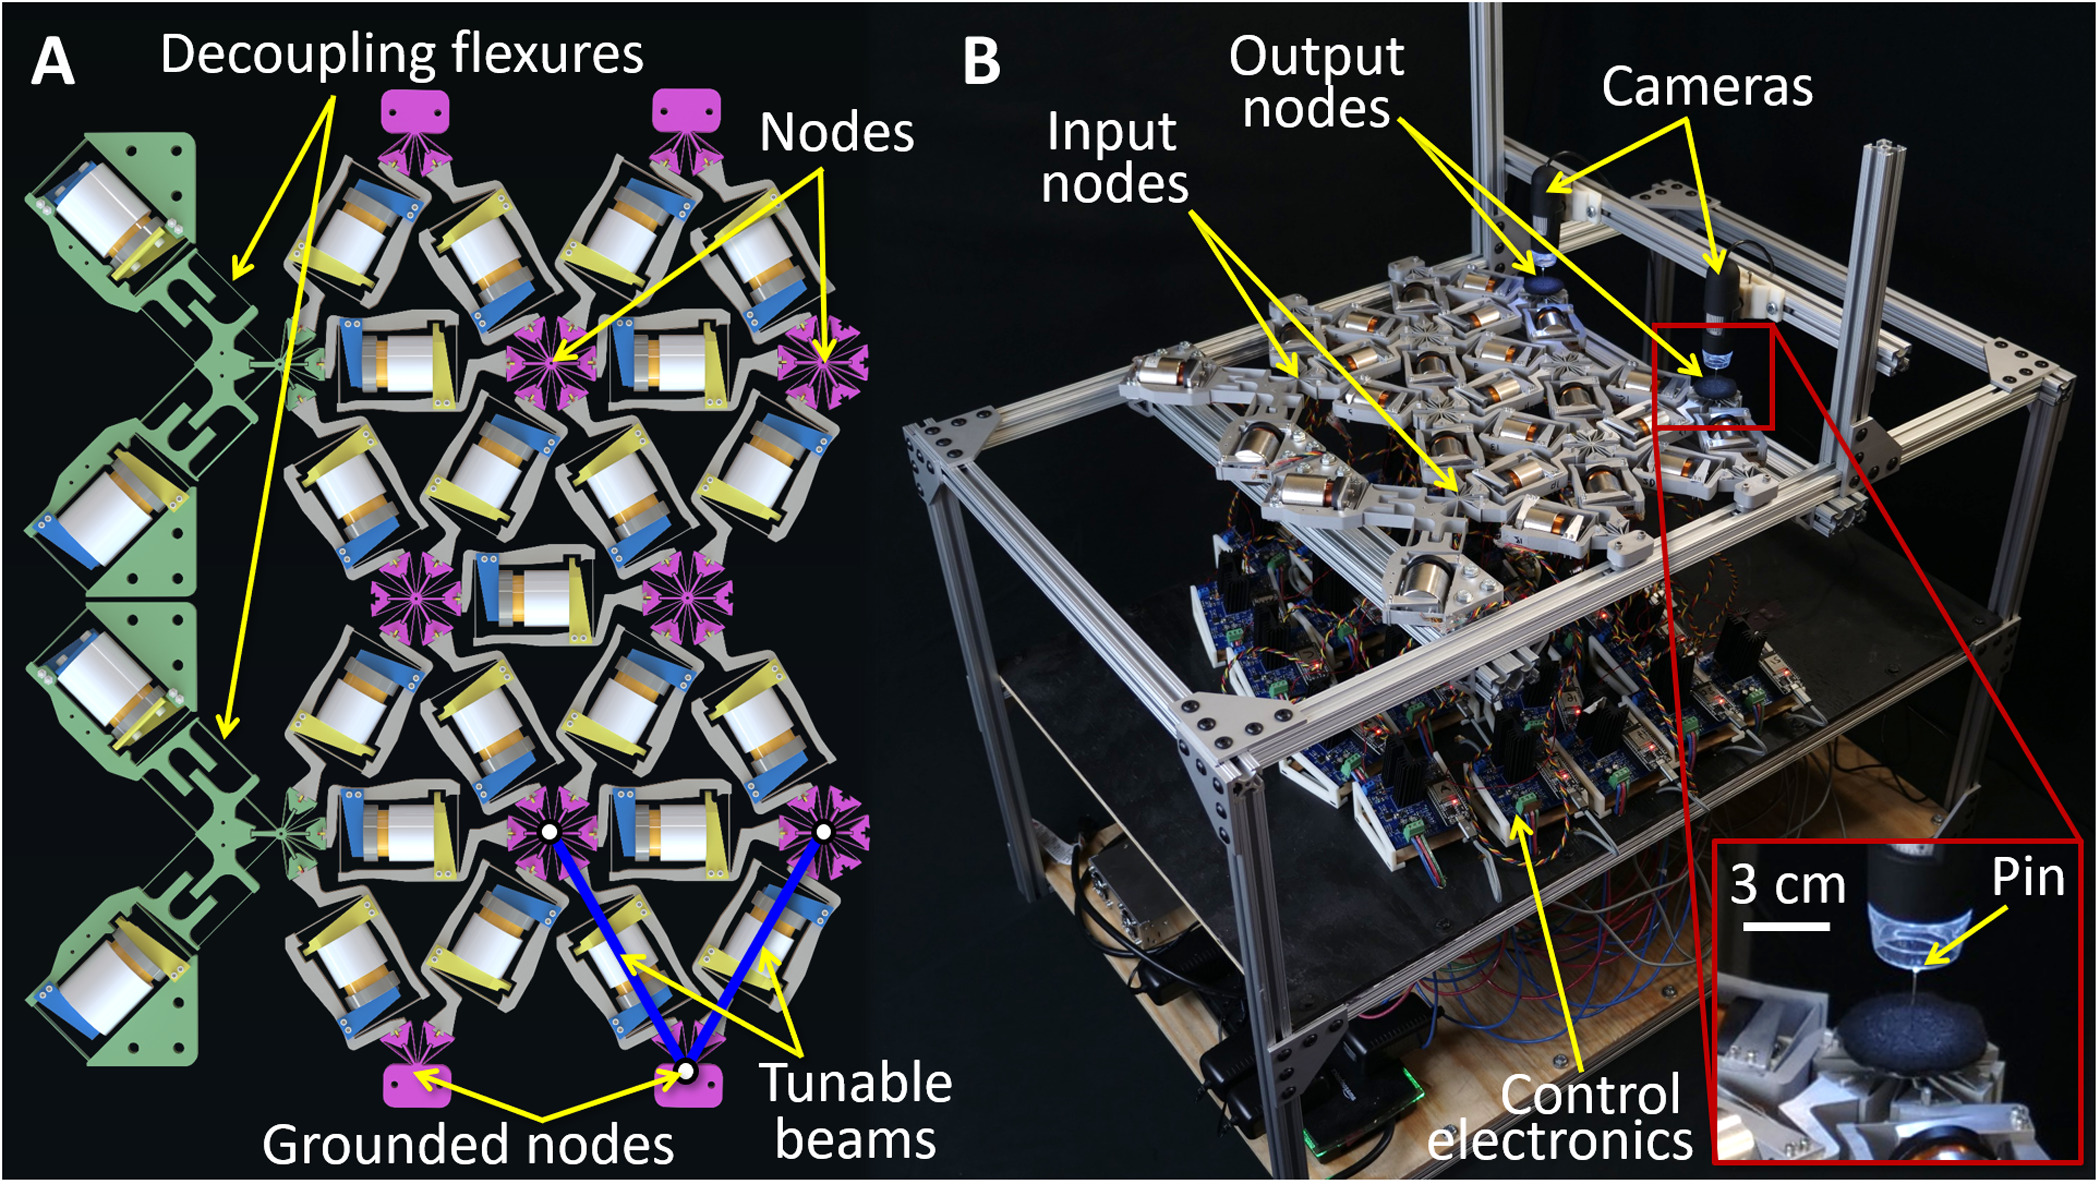
\includegraphics[width=0.65\linewidth]{bilder/mnn2-1.jpg}
    \caption{Mechanische Umsetzung eines MNN (Abb. von \cite{Lee2022})}
    \label{fig:mnn2-1}
\end{figure}

Durch ihre Eigenschaften könnten MNNs viele Verwendungszwecke haben, von der Optimierung von Flugzeugflügeln abhängig von aktuellen Gegebenheiten wie Windstärke und -winkel \cite[2]{Lee2022} über Optimierung der Schockabsorption von Schutzwesten bis zur dynamischen Änderung der Resonanzfrequenz eines Gebäudes zum Schutz gegen Erdbeben \cite[9]{Hopkins2023}.
Wenn es möglich ist, die Resonanz auf Schwingungen eines MNNs zu trainieren, könnte man dies auch für einbruchsichere Brücken oder vielleicht sogar bessere Musikinstrumente nutzen.

In diesem Projekt wollen wir verschiedene Optimierungsalgorithmen für MNNs vergleichen.
% und analysieren, wie viele verschiedene Verhaltensweisen gleichzeitig gelernt werden können. 
Da wir nichts passendes finden konnten, wollen wir zuerst eine eigene Programmbibliothek zur Simulation, Optimierung, Bewertung und Visualisierung von MNNs erstellen.
Diese soll nutzerfreundlich und öffentlich sein, damit wir und andere sie als Basis für weiterführende Projekte nutzen können.

Zur Bewertung der Optimierungsalgorithmen und -parameter sollen MNNs simuliert werden.
Ziel dieses Projektes ist es aufgrund des hohen Aufwands nicht, ein MNN selbst physisch umzusetzen;
es wird jedoch davon ausgegangen, dass ein Vergleich der Verfahren in einer Simulation auch korrekte Aussagen über das physische Trainieren liefern wird und ein \enquote{Vortrainieren} eines physischen MNN mit einer Simulation die Gesamtzeit des Trainierens verkürzen kann, somit also auch die in einer Simulation verwendeten Optimierungsverfahren relevant sind.

% \begin{figure}
%     \centering
%     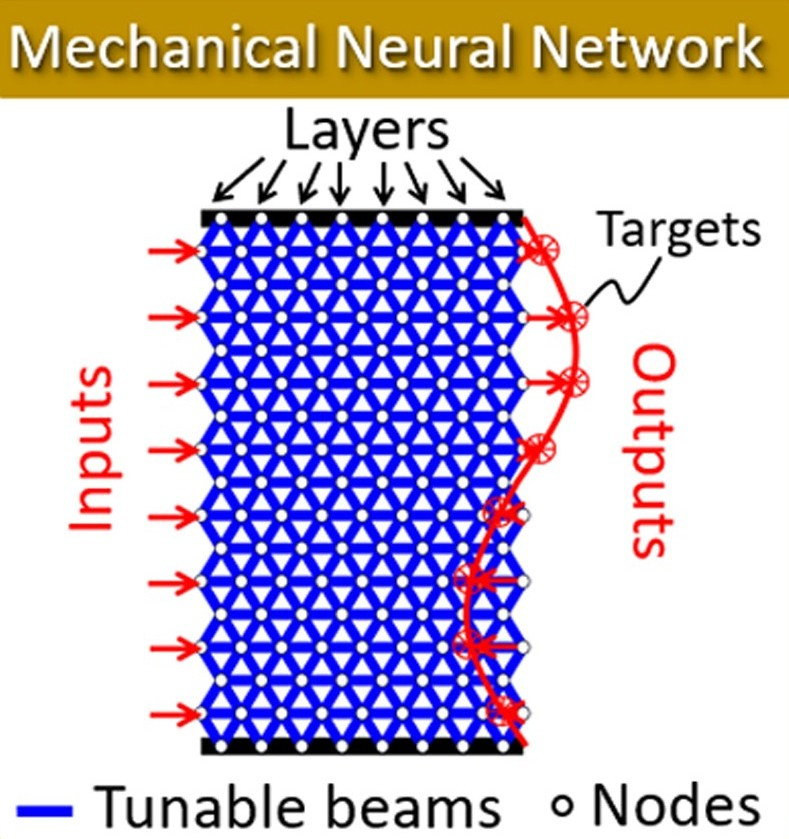
\includegraphics[width=0.4\linewidth]{bilder/mnn1-1.jpg}
%     \caption{Repräsentation eines MNN (von \cite{Lee2022})}
%     \label{fig:mnn1-1}
% \end{figure}